\section{Enriquecimiento Analítico: Web Scraping de Salud Pública y API Climática}
\label{sec:bonos}

Esta sección documenta la integración de las dos fuentes externas de enriquecimiento territorial y ambiental (previstas en el numeral 2.4 y conectadas en Spark con los conjuntos principales de arrestos, colisiones y pobreza): la extracción automatizada de tasas de incidencia de cáncer por vecindario mediante \textit{web scraping} del \textit{NYS Department of Health} y la extracción de series meteorológicas diarias mediante API REST (\textit{OpenWeather One Call 3.0 / Open-Meteo}).

\subsection{Web Scraping: Tasas de Cáncer por Vecindario PUMA (NYS Department of Health)}
\label{subsec:bono_cancer}

La fuente consultada es el tablero oficial \textit{``Rate by PUMA''} del \textit{New York State Cancer Registry} \cite{nys_cancer_registry_2026}, donde los vecindarios de Nueva York se delimitan mediante unidades censales PUMA (\textit{Public Use Microdata Areas}), equivalentes aproximadamente a los distritos comunitarios de la ciudad. Dado que la página institucional incrusta una vista dinámica de \textit{Tableau Public} en lugar de una tabla HTML estática, el flujo programado en Python ejecuta cuatro etapas: (i) descarga el documento HTML de \texttt{ratebyPUMA.htm} mediante \texttt{requests}, (ii) identifica mediante expresiones regulares la ruta del libro (\texttt{cancerstatisticreportcounty}) y la hoja (\texttt{7\_RatebyPUMA}) a partir de los metadatos de vista previa de Tableau, (iii) descarga directamente el flujo CSV subyacente desde el servidor de \textit{Tableau Public} y (iv) normaliza las columnas para conservar la serie agregada (\textit{All Sites Combined}, ambos sexos) para cada uno de los $55$ PUMA de la Ciudad de Nueva York, almacenando además una copia en caché local (\texttt{cancer\_tasas\_puma\_nyc.csv}) para garantizar reproducibilidad en entornos de clúster con acceso restringido.

\subsection{Resultados del Scraping: Distribución de Tasas por PUMA y Condado}
\label{subsec:bono_puma}

Se extrajeron exitosamente los registros de los $55$ PUMA de la metrópoli ($10$ en el Bronx, $18$ en Brooklyn, $10$ en Manhattan, $14$ en Queens y $3$ en Staten Island). La tasa promedio de incidencia en los vecindarios de la ciudad es de $423.5$ casos por cada $100,000$ habitantes, con un rango entre $355.7$ (\textit{Bushwick}, Brooklyn) y $541.0$ (\textit{South Shore}, Staten Island). La Tabla \ref{tab:top10_puma_cancer} presenta los diez vecindarios con mayor tasa y la Figura \ref{fig:bono_cancer_puma} ilustra la dispersión intraterritorial por condado junto con el ranking de los diez primeros PUMA.

\begin{table}[H]
\centering
\small
\caption{Top 10 de vecindarios PUMA con mayor tasa de incidencia de cáncer (todos los sitios combinados, ambos sexos).}
\label{tab:top10_puma_cancer}
\begin{tabularx}{\linewidth}{c l X r}
\toprule
\textbf{\#} & \textbf{Condado} & \textbf{PUMA (vecindario)} & \textbf{Tasa por 100,000 hab.} \\
\midrule
1 & Staten Island & South Shore & 541.0 \\
2 & Staten Island & Mid-Island & 512.7 \\
3 & Staten Island & North Shore & 490.4 \\
4 & Brooklyn & Sheepshead Bay \& Gravesend (East) & 476.1 \\
5 & Queens & The Rockaways & 464.4 \\
6 & Manhattan & Upper East Side \& Roosevelt Island & 460.9 \\
7 & Brooklyn & Coney Island \& Brighton Beach & 459.7 \\
8 & Manhattan & Midtown, East Midtown, \& Flatiron & 450.6 \\
9 & Brooklyn & Park Slope \& Carroll Gardens & 450.0 \\
10 & Brooklyn & Bay Ridge \& Dyker Heights & 449.9 \\
\bottomrule
\end{tabularx}
\end{table}

\begin{figure}[H]
    \centering
    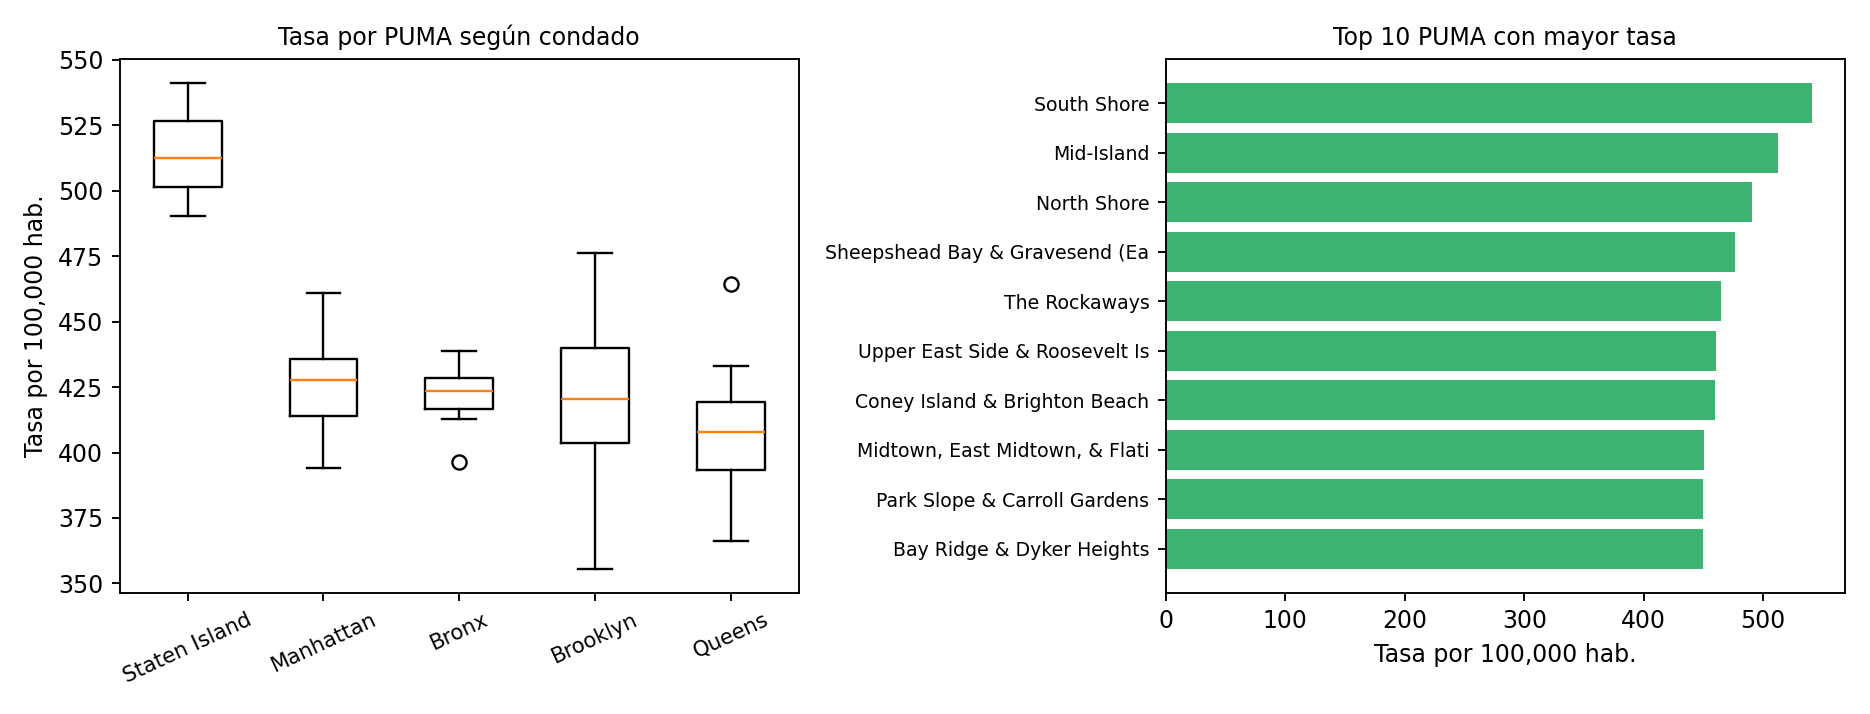
\includegraphics[width=0.92\textwidth]{imagenes/imaged.png}
    \caption{Distribución de la tasa de incidencia de cáncer por PUMA según condado (izquierda) y top 10 de PUMA con mayor tasa (derecha).}
    \label{fig:bono_cancer_puma}
\end{figure}

\subsection{Cruce Multidimensional: Cáncer, Pobreza, Arrestos y Colisiones por Condado}
\label{subsec:bono_cruce}

La Tabla \ref{tab:cruce_condado_cancer} y la Figura \ref{fig:bono_cruce_cancer} integran la tasa promedio de incidencia de cáncer por condado con la proporción de pobreza y las tasas estandarizadas de arrestos y colisiones por cada $100,000$ habitantes calculadas en la Sección \ref{sec:limpieza_transformacion} (Tabla \ref{tab:tasas_100k}). Se observa un contraste demográfico revelador: Staten Island exhibe el mayor promedio de incidencia de cáncer ($514.7$ por $100,000$ hab., asociado a una estructura poblacional de mayor edad media y mayor detección diagnóstica) pero simultáneamente presenta la menor tasa de arrestos ($1,101.2$), la menor tasa de colisiones viales ($666.4$) y una de las menores tasas de pobreza ($13.8\%$). Por el contrario, el Bronx registra la mayor pobreza ($25.8\%$) y la mayor tasa de arrestos ($2,354.5$), mientras que Brooklyn lidera la tasa de siniestralidad vial ($1,051.4$), manteniendo ambos tasas promedio de cáncer cercanas a la media urbana ($421.7$ y $421.1$, respectivamente).

\begin{table}[H]
\centering
\scriptsize
\renewcommand{\arraystretch}{1.2}
\caption{Cruce por condado entre tasa promedio de cáncer (PUMA), pobreza y tasas de arrestos y colisiones por 100,000 habitantes.}
\label{tab:cruce_condado_cancer}
\begin{tabularx}{\linewidth}{l c >{\centering\arraybackslash}X >{\centering\arraybackslash}X >{\centering\arraybackslash}X >{\centering\arraybackslash}X}
\toprule
\textbf{Condado} & \textbf{N.$^{\circ}$ PUMA} & \textbf{Tasa cáncer (prom.)} & \textbf{Pobreza (\%)} & \textbf{Arrestos / 100k} & \textbf{Colisiones / 100k} \\
\midrule
Staten Island & 3 & 514.7 & 13.8 & 1,101.2 & 666.4 \\
Manhattan & 10 & 427.1 & 13.8 & 2,064.1 & 931.9 \\
Bronx & 10 & 421.7 & 25.8 & 2,354.5 & 885.5 \\
Brooklyn & 18 & 421.1 & 18.3 & 1,687.6 & 1,051.4 \\
Queens & 14 & 405.9 & 15.8 & 1,290.8 & 970.3 \\
\bottomrule
\end{tabularx}
\end{table}

\begin{figure}[H]
    \centering
    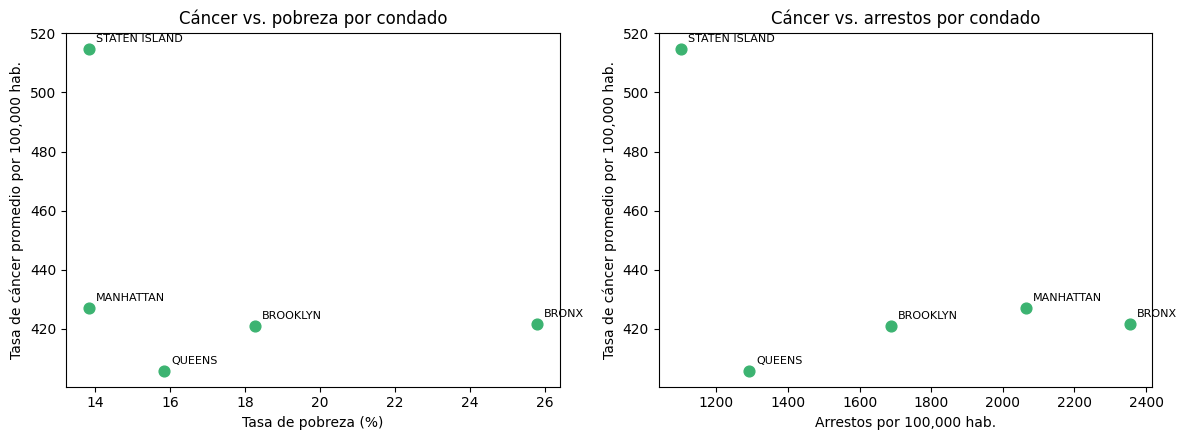
\includegraphics[width=0.9\textwidth]{imagenes/imagee.png}
    \caption{Tasa promedio de cáncer por condado frente a la tasa de pobreza (izquierda) y a los arrestos por 100,000 habitantes (derecha).}
    \label{fig:bono_cruce_cancer}
\end{figure}

\subsection{API Climática: Extracción y Caracterización Meteorológica Diaria en NYC}
\label{subsec:bono_api_clima}

El pipeline consulta las variables meteorológicas diarias para el centro geográfico de la Ciudad de Nueva York ($\text{lat } 40.7128, \text{lon } -74.0060$) cubriendo exactamente las $546$ fechas comprendidas entre el 1 de enero de 2025 (año completo de referencia de colisiones) y el 30 de junio de 2026 (horizonte del conjunto de arrestos y conjunto de prueba de los modelos). El conector soporta el endpoint \texttt{day\_summary} de \textit{OpenWeather One Call API 3.0} \cite{openweather_onecall_2026} y el archivo histórico de \textit{Open-Meteo} \cite{openmeteo_historical_2026}, persistiendo las $546$ observaciones diarias en \texttt{clima\_nyc\_diario.csv} con temperatura mínima y máxima ($^\circ\text{C}$), precipitación total ($\text{mm}$) y velocidad máxima del viento ($\text{m/s}$).

La Tabla \ref{tab:clima_mensual_nyc} y la Figura \ref{fig:bono_clima_diario} sintetizan el comportamiento mensual y diario extraído: julio de 2025 presentó la mayor temperatura máxima media diaria ($31.8\,^\circ\text{C}$) y febrero de 2026 la mínima media diaria más baja ($-7.4\,^\circ\text{C}$), mientras que mayo de 2025 fue el mes de mayor precipitación acumulada ($201.1\text{ mm}$ en $16$ días con lluvia $\ge 1\text{ mm}$).

\begin{table}[H]
\centering
\scriptsize
\caption{Resumen mensual del clima extraído en NYC (enero de 2025 a junio de 2026).}
\label{tab:clima_mensual_nyc}
\setlength{\tabcolsep}{4pt}
\begin{tabularx}{\linewidth}{c c >{\centering\arraybackslash}X >{\centering\arraybackslash}X >{\centering\arraybackslash}X c c}
\toprule
\textbf{Mes} & \textbf{Días} & \textbf{T.~mín. ($^{\circ}$C)} & \textbf{T.~máx. ($^{\circ}$C)} & \textbf{Precip. (mm)} & \textbf{Días lluvia} & \textbf{Viento (m/s)} \\
\midrule
2025-01 & 31 & $-5.3$ & $1.3$ & $30.3$ & 6 & $8.3$ \\
2025-02 & 28 & $-3.2$ & $4.1$ & $79.4$ & 11 & $8.0$ \\
2025-03 & 31 & $2.1$ & $12.6$ & $162.5$ & 10 & $8.5$ \\
2025-04 & 30 & $7.3$ & $17.1$ & $73.1$ & 10 & $8.4$ \\
2025-05 & 31 & $12.7$ & $21.1$ & $201.1$ & 16 & $7.1$ \\
2025-06 & 30 & $18.9$ & $28.8$ & $74.9$ & 12 & $5.8$ \\
2025-07 & 31 & $22.4$ & $31.8$ & $111.4$ & 15 & $6.3$ \\
2025-08 & 31 & $18.4$ & $28.5$ & $23.8$ & 6 & $6.3$ \\
2025-09 & 30 & $16.6$ & $25.6$ & $119.5$ & 9 & $5.7$ \\
2025-10 & 31 & $9.7$ & $18.4$ & $110.5$ & 7 & $7.9$ \\
2025-11 & 30 & $3.6$ & $11.2$ & $49.7$ & 9 & $7.8$ \\
2025-12 & 31 & $-3.9$ & $3.3$ & $79.9$ & 8 & $8.5$ \\
2026-01 & 31 & $-6.2$ & $1.1$ & $68.7$ & 6 & $8.3$ \\
2026-02 & 28 & $-7.4$ & $0.7$ & $53.2$ & 6 & $9.2$ \\
2026-03 & 31 & $2.2$ & $12.3$ & $106.9$ & 12 & $9.2$ \\
2026-04 & 30 & $7.6$ & $18.1$ & $72.7$ & 13 & $6.5$ \\
2026-05 & 31 & $12.9$ & $23.1$ & $98.2$ & 11 & $7.6$ \\
2026-06 & 30 & $18.9$ & $29.0$ & $95.0$ & 14 & $8.7$ \\
\bottomrule
\end{tabularx}
\end{table}

\begin{figure}[H]
    \centering
    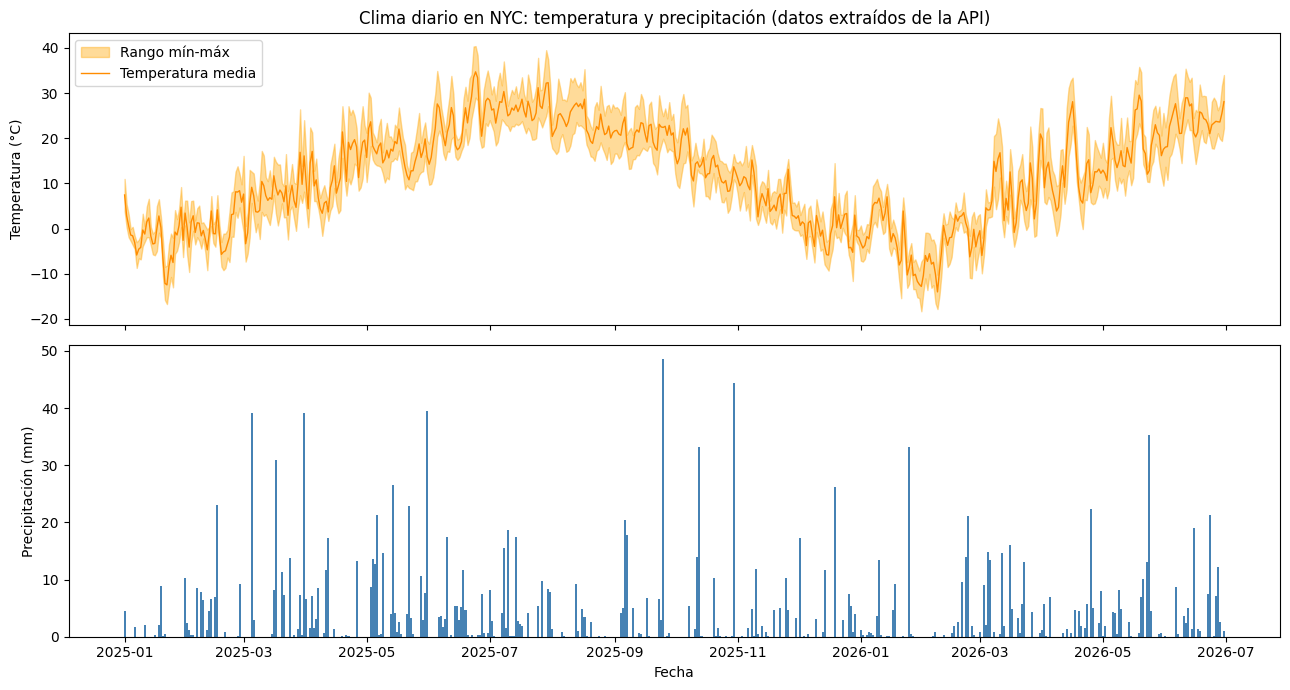
\includegraphics[width=0.88\textwidth]{imagenes/imagef.png}
    \caption{Temperatura (banda mínima--máxima y media diaria) y precipitación diaria en NYC (enero de 2025 a junio de 2026).}
    \label{fig:bono_clima_diario}
\end{figure}

\subsection{Cruce Distribuido en Spark: Clima frente a Colisiones y Arrestos Diarios}
\label{subsec:bono_cruce_clima}

Para conectar las variables meteorológicas con los indicadores de negocio (Objetivo 3), la serie climática se convirtió a un DataFrame distribuido de Spark (\texttt{clima\_sdf}) definiendo la temperatura media diaria $\texttt{temp\_media\_c} = (\texttt{temp\_min\_c} + \texttt{temp\_max\_c})/2$ y el indicador binario de día lluvioso ($\texttt{lluvia} = \mathbb{I}(\texttt{precip\_mm} \ge 1)$). Posteriormente, se efectuó un \texttt{inner join} por fecha con las colisiones diarias agregadas de 2025 ($365$ días) y con los arrestos diarios del primer semestre de 2026 ($181$ días). La Tabla \ref{tab:correlacion_clima} y la Figura \ref{fig:clima_vs_colisiones_arrestos} presentan las correlaciones de Pearson obtenidas.

\begin{table}[H]
\centering
\small
\renewcommand{\arraystretch}{1.2}
\caption{Correlación de Pearson entre variables meteorológicas diarias y el volumen de colisiones, heridos y arrestos.}
\label{tab:correlacion_clima}
\begin{tabular}{l c r r r}
\toprule
\textbf{Indicador Diario} & \textbf{Días ($n$)} & \textbf{Temp.~media ($^{\circ}$C)} & \textbf{Precipitación (mm)} & \textbf{Viento máx. (m/s)} \\
\midrule
Colisiones diarias (2025) & 365 & $+0.301$ & $+0.077$ & $-0.132$ \\
Personas heridas por día (2025) & 365 & $\mathbf{+0.469}$ & $+0.051$ & $-0.159$ \\
Arrestos diarios (2026-I) & 181 & $+0.134$ & $\mathbf{-0.306}$ & $-0.190$ \\
\bottomrule
\end{tabular}
\end{table}

\begin{figure}[H]
    \centering
    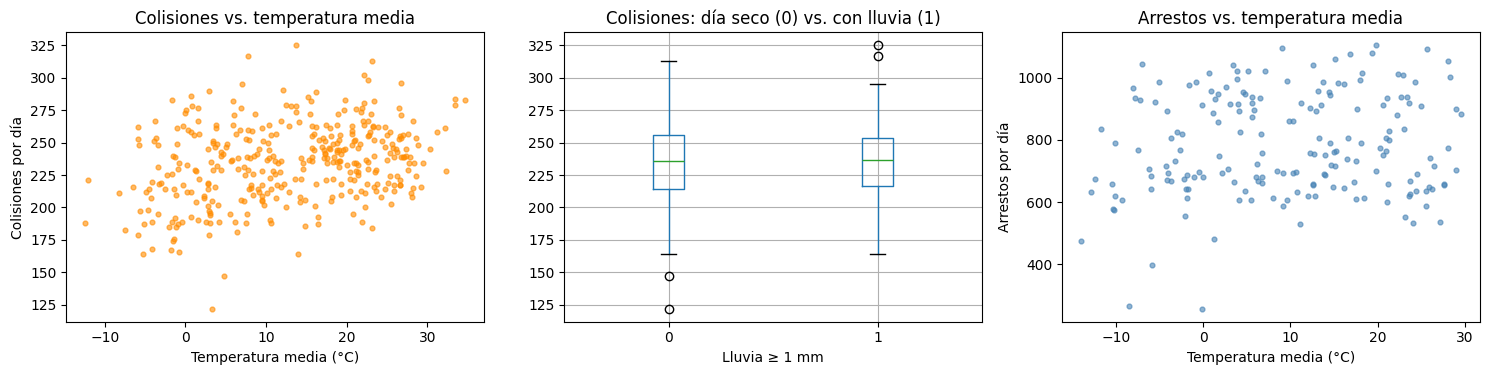
\includegraphics[width=0.95\textwidth]{imagenes/fig_cell_92_1.png}
    \caption{Relación diaria entre temperatura media, condición de lluvia ($\ge 1\text{ mm}$) y volumen de colisiones y arrestos en NYC.}
    \label{fig:clima_vs_colisiones_arrestos}
\end{figure}

\noindent \textbf{Interpretación de negocio:} En 2025, la temperatura media diaria presentó una correlación positiva de $r = +0.301$ con el conteo de colisiones y de $r = +0.469$ con el total diario de personas heridas, explicada por el incremento estacional de flujos peatonales, ciclistas y motociclistas durante la primavera y el verano. El promedio diario en los $119$ días con lluvia fue de $235.1$ colisiones frente a $234.0$ en los $246$ días secos. Por su parte, en el primer semestre de 2026, los arrestos diarios exhibieron una correlación negativa moderada con la precipitación ($r = -0.306$), evidenciando que los eventos de lluvia reducen la actividad en espacio público y las detenciones en vía abierta.
